\begin{Problem}{Coffee and Chicken}{1}

据说,“Coffee Chicken”在组队的时候,ICPC集训队刚好购置了福利咖啡机,所以起了这个名字。我们不禁感叹:ICPC集训队的福利真实好!我们都要做Coffee Chicken的粉丝!

这一次,咖啡鸡把自己藏在了一个$n\times m$的字符矩阵里(字符矩阵由大写字母构成),并且希望我们找出隐藏的“咖啡鸡”——从矩阵的某个格子出发,向如下图所示的8个方向,如果能读出\texttt{COFFEE}或\texttt{CHICKEN},则认为找到了一个单词。

\begin{figure}[h]
  \center
  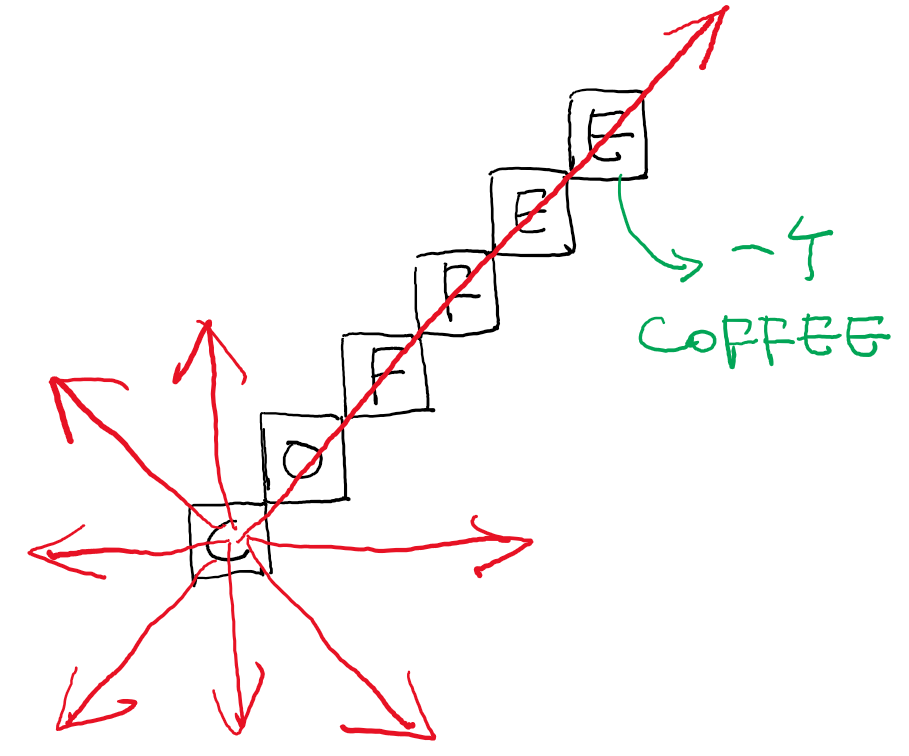
\includegraphics[width=6cm]{src/cac/coffeechicken.png}
\end{figure}

你的任务是统计单词\texttt{COFFEE}和\texttt{CHICKEN}出现的次数。

\subsection*{输入格式}

输入数据第一行包含两个整数 $n$, $m$ ($1\le n,m\le 100$)。接下来$n$行,每行$m$个用空格分隔开的大写字母描述了一个字符矩阵。

\subsection*{输出格式}

输出两行:

\begin{enumerate}
\item 第一行格式:$\texttt{COFFEE x $x$}$
\item 第二行格式:$\texttt{CHICKEN x $y$}$
\end{enumerate}

其中$x$, $y$分别是字符矩阵中\texttt{COFFEE}和\texttt{CHICKEN}出现的次数。

\exmpv{01-sample}
\exmpv{02-sample}

\end{Problem}
